\documentclass[a4paper,11pt]{article}

% Kodovani (cestiny) v dokumentu: utf-8
%\usepackage[cp1250]{inputenc}	% Omezena stredoevropska kodova stranka, pouze MSW.
\usepackage[utf8]{inputenc}	% Doporucujeme pouzivat UTF-8 (unicode).

\usepackage[margin=2cm]{geometry}
\newtoks\jmenopraktika \newtoks\jmeno \newtoks\datum
\newtoks\obor \newtoks\skupina \newtoks\rocnik \newtoks\semestr
\newtoks\cisloulohy \newtoks\jmenoulohy
\newtoks\tlak \newtoks\teplota \newtoks\vlhkost

\jmenopraktika={Fyzikální praktikum 1}
\jmeno={Lukáš Lejdar}
\datum={22. října 2024}
\obor={F}
\skupina={Út 16:00}

\cisloulohy={10}
\jmenoulohy={Polarizace světla}

\tlak={101{,}35}
\teplota={21,1}
\vlhkost={47,7}


%%%%%%%%%%% Uzitecne balicky:
\usepackage[czech]{babel}

\usepackage{graphicx}
\usepackage{amsmath}
\usepackage{xspace}
\usepackage{url}
\usepackage{indentfirst}
\usepackage{wrapfig}
\usepackage{xcolor}
\usepackage{subfig}
\usepackage{subcaption}
\usepackage{enumitem}
\usepackage{tikzsymbols}
\usepackage{newfloat}
\usepackage{siunitx}


\DeclareFloatingEnvironment[fileext=lof]{graph}
\captionsetup[graph]{labelformat=simple, labelsep=colon, name=Graf}
\newcommand{\sperc}{\text{\footnotesize\%}}


%%%%%% Zamezeni parchantu:
\widowpenalty 10000 \clubpenalty 10000 \displaywidowpenalty 10000
%%%%%% Parametry pro moznost vsazeni vetsiho poctu obrazku na stranku
\setcounter{topnumber}{3}	  % max. pocet floatu nahore (specifikace t)
\setcounter{bottomnumber}{3}	  % max. pocet floatu dole (specifikace b)
\setcounter{totalnumber}{6}	  % max. pocet floatu na strance celkem
\renewcommand\topfraction{0.9}	  % max podil stranky pro floaty nahore
\renewcommand\bottomfraction{0.9} % max podil stranky pro floaty dole
\renewcommand\textfraction{0.1}	  % min podil stranky, ktery musi obsahovat text
\intextsep=8mm \textfloatsep=8mm  %\intextsep pro ulozeni [h] floatu a \textfloatsep pro [b] or [t]

% Tecky za cisly sekci:
\renewcommand{\thesection}{\arabic{section}.}
\renewcommand{\thesubsection}{\thesection\arabic{subsection}.}
% Jednopismenna mezera mezi cislem a nazvem kapitoly:
\makeatletter \def\@seccntformat#1{\csname the#1\endcsname\hspace{1ex}} \makeatother
%
\newcommand{\vsn}[4]{\ensuremath{#1 =} #2(#3)\,#4}
\newcommand{\vrn}[6]{\ensuremath{#1 =} (#2 $\pm$ #3)\,#4 ($p=$ #5\,\%, $\nu=$ #6)}

\newcommand*\circled[1]{\tikz[baseline=(char.base)]{
		\node[shape=circle,draw,inner sep=1pt] (char) {#1};}}

%%%%%%%%%%%%%%%%%%%%%%%%%%%%%%%%%%%%%%%%%%%%%%%%%%%%%%%%%%%%%%%%%%%%%%%%%%%%%%%
% Zacatek dokumentu
%%%%%%%%%%%%%%%%%%%%%%%%%%%%%%%%%%%%%%%%%%%%%%%%%%%%%%%%%%%%%%%%%%%%%%%%%%%%%%%

\begin{document}

\thispagestyle{empty}

{
\begin{center}
\sf 
{\Large Ústav fyziky a technologií plazmatu Přírodovědecké fakulty Masarykovy univerzity} \\
\bigskip
{\huge \bfseries FYZIKÁLNÍ PRAKTIKUM} \\
\bigskip
{\Large \the\jmenopraktika}
\end{center}

\bigskip

\sf
\noindent
\setlength{\arrayrulewidth}{1pt}
\begin{tabular*}{\textwidth}{@{\extracolsep{\fill}} l l}
\large {\bfseries Zpracoval:}  \the\jmeno & \large  {\bfseries Naměřeno:} \the\datum\\[2mm]
\large  {\bfseries Obor:} \the\obor  \hspace{40mm}  {\bfseries Skupina:} \the\skupina %
&\large {\bfseries Testováno:}\\
\\
\hline
\end{tabular*}
}

\bigskip

{
\sf
\noindent \begin{tabular}{p{4cm} p{0.6\textwidth}}
\Large  Úloha č. {\bfseries \the\cisloulohy:} \par
\smallskip
$T=\the\teplota$~$^\circ$C \par
$p=\the\tlak$~kPa \par
&\Large \bfseries \the\jmenoulohy  \\[2mm]
\end{tabular}
}

\vspace{-10pt}

\section{Úvod}

V úloze budu měřit optické vlastnosti roztoku sacharózy, pokusím se ověřit Malusův zákon a změřím polarizační schopnosti reálných polaroidů.
 
\subsection{Měření indexu lomu na refraktometru}

Základní částí přístroje jsou 2 hranoly $ H_1 $ a $ H_2 $. Světlo vstupuje stěnou $ EF $ hranolu, rozptýlí se na zamatované ploše $ ED $ a vchází do měřené látky, která je rozprostřená mezi hranoly. Na ploše $ BC $ tím vzniká světlé a tmavé rozhraní, kam světlo kvůli indexu lomu měřené látky už nemůže. Tuto stranu jde zároveň pozorovat okulkárem, ze kterého lze přímo odečíst index lomu. V případě, že měřený vzorek je roztok sacharózy, jde odečítat i jeho koncentraci.

\begin{figure}[htpb]
    \centering
    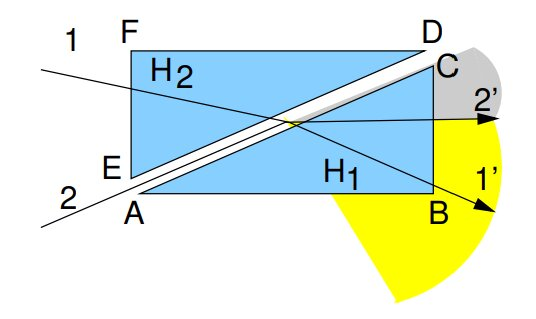
\includegraphics[width=0.4\textwidth]{refraktometr.jpg}
    \caption{Optický princip dvojhranolového refraktometru}
\end{figure}

\subsection{Polarimetr}

Schématicky je polarimetr znázorněný na obrázku 2. Soustava zdroje $ (Z) $, kolimátoru $ (K) $ a poloarizátoru $ (P) $ dohromady vytvoří lineárně polarizovaný paprsek dopadající na vzorek $ V $, který dál prochází na analyzátor $ (A) $. Jsou-li zkřížené kmitové roviny polarizátoru a analyzátoru, bude nastávat minimum intenzity osvětlení zorného pole, které jde pozorovat v dalekohledu $ (D) $. Úhel stočení analyzátoru potom odpovídá stočení polarizace pozorovanou látkou, když od ní odečtu stočení bez vzorku.

Úhel stočení kmitové roviny po průchodu kapalinou je přímo úměrný koncentraci aktivní látky $ c $ a délky vzorku $ d $. 

\begin{equation}
\alpha = [\alpha] cd
\end{equation}

\begin{figure}[htpb]
    \centering
    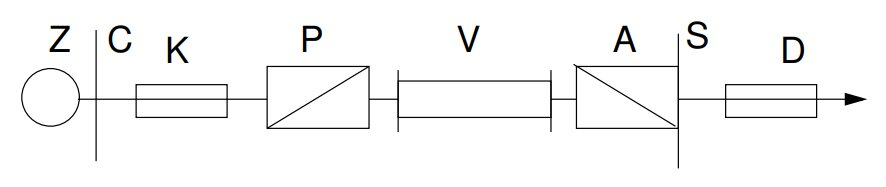
\includegraphics[width=0.5\textwidth]{polarimetr.jpg}
    \caption{Polarimetr}
\end{figure}

\subsection{Ověření Malusova zákona}

    Schéma Malusova experimentu je znázorněné na obrázku 3. Lineárně polarizované světlo z polarizátoru $ (P) $ dopadá na analyzátor $ (A) $, který je taky polarizátor jen v jiném směru. Když úhel mezi polarizacemi $ \vec{E}_P $ a $ \vec{E}_A $ označím $ \varphi $, pak podle Malusova zákona platí

\begin{equation}
E_A = E_P \cos \varphi
\end{equation}

\noindent
V případě nedokonalých polarizátorů bude část světla pronikat i při zkřížených rovinách. Malusův zákon pak můžeme upravit pro měřené intenzity na

\begin{equation}
I = I_{\text{min}} + (I_{\text{max}} - I_{\text{min}}) \cos^2 \alpha
\end{equation}

\begin{figure}[htpb]
    \centering
    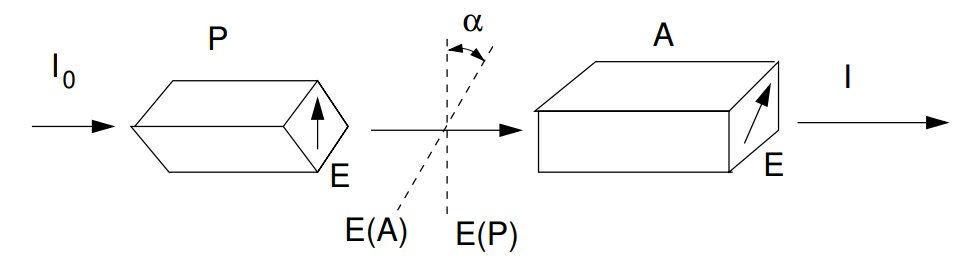
\includegraphics[width=0.6\textwidth]{malus_schema.jpg}
    \caption{Schéma Malusova pokusu}    
\end{figure}

Takové nedokonale polarizované světlo je možné rozložit na z části polarizované (intenzita $ I_p $) a z části nepolarizované ($ I_n $). Zavadíme proto veličinu stupeň polarizace

\begin{equation}
V = \frac{I_p}{I_p + I_n}
\end{equation}

\noindent
Pokud polarizátor budu považovat za nedokonalý a analyzátor za dokonalý, bude platit

\begin{align}
    I_{\text{max}} &= I_p + \frac{I_n}{2} \\
    I_{\text{min}} &= \frac{I_n}{2}
\end{align}

\noindent
odkud můžu dosadit do vztahu (4).

\begin{equation}
V = \frac{I_{\text{max}} - I_{\text{min}}}{I_{\text{max}} + I_{\text{max}}}
\end{equation}

\newpage

\section{Výsledky měření}

\subsection{Měření indexu lomu a stáčivosti roztoku sacharózy}

Připravil jsem roztoky sacharózy o koncentracích $ 15 \% $, $ 10 \% $, $ 5 \% $ a destilovanou vodu a určil jejich index lomu i reálnou koncentraci pomocí refraktometru. Těmito roztoky jsem potom naplnil kyvety o délce $ d = 0.1 $ m a měřil jejich optickou aktivitu polarimetrem. Čistá destilovaná voda by měla mít nulovou stáčivost, takže v jejím případě budu odečítat z polarimetru bez vzorku.

\vspace{-5pt}

\begin{table}[htpb]
    \centering
    \resizebox{\textwidth}{!}{% 
    \begin{tabular}{ccc ccc ccc ccc}
        \hline\hline
        \multicolumn{3}{c|}{$ \odot $ $ 15 \sperc $ sacharózy} & \multicolumn{3}{c|}{$ \odot $ $ 10 \sperc $ sacharózy} & \multicolumn{3}{c|}{$ \odot $ $ 5 \sperc $ sacharózy} & \multicolumn{3}{c}{destilovaná voda} \\
        $ c $ ($ \sperc $) & n & \multicolumn{1}{c|}{$ \varphi $ $ (^{\circ}) $} & $ c $ ($ \sperc $) & n & \multicolumn{1}{c|}{$ \varphi $ $ (^{\circ}) $} & $ c $ ($ \sperc $) & n & \multicolumn{1}{c|}{$ \varphi $ $ (^{\circ}) $} & $ c $ ($ \sperc $) & n & $ \varphi $ $ (^{\circ}) $ \\\hline
        14.0 & 1.3540 & 10.40 & 8.4 & 1.3451 & 6.10 & 3.6 & 1.3382 & 2.90 & -0.5 & 1.3221 & 0.00 \\
        14.1 & 1.3543 & 10.45 & 8.4 & 1.3452 & 6.10 & 3.7 & 1.3383 & 2.95 & -0.5 & 1.3322 & 0.05 \\
        14.0 & 1.3541 & 10.40 & 8.5 & 1.3453 & 6.15 & 3,5 & 1.3380 & 2.90 & -0.5 & 1.3319 & 0.00 \\\hline
\small 14.03(3) & \small 1.3541(1) & \small 10.42(2) & \small 8.43(3) & \small 1.3452(1) & \small 6.12(2) & \small 3.60(6) & \small 1.3382(1) & \small 2.92(2) & \small -0.5 & \small 1.329(3) & \small 0.02(2) \\
        \hline\hline
    \end{tabular} 
    }
    \caption{Měření optických vlastností roztoků sacharózy}
\end{table}

\vspace{-15pt}

V tabulce 1 je výsledná koncentrace destilované vody záporná, což by nemělo být možné. Naznačuje to malou chybu v seřízení přístroje, se kterou se vypořádám odečtením hodnoty $ c_{0} = -0.5 \sperc $ od všech ostatních. S takto upravenými hodnotami spočítám stáčivost roztoku sacharózy $ [\alpha] $ podle vztahu (1) a zprůměrováním pro všechny roztoky dostávám

\begin{equation*}
[\alpha] = 70.2 \pm 0.4 \ \ \frac{\text{cm}^{3}}{\text{g dm}}
\end{equation*}

\subsection{Ověření Malusova zákon}

\begin{wraptable}{r}{0.45\textwidth}
    \vspace{-10pt}
    \centering
    \begin{tabular}{ccccc}
        \hline\hline
        & \multicolumn{2}{c|}{bílé světlo} & \multicolumn{2}{c}{$\lambda = 671$ nm} \\
        & $ \varphi $ ($ ^{\circ} $) & \multicolumn{1}{c|}{$ I $ mA}  & $ \varphi $ ($ ^{\circ} $) & $ I $ $ \mu $A \\\hline
        min & 71 & 1.025 & 74 & 0.91 \\
        max & 162 & 1.271 & 167 & 5.07 \\\hline
        V =  & \multicolumn{2}{c}{0.1071} & \multicolumn{2}{c}{0.6957} \\
        \hline\hline
    \end{tabular}
    \caption{Maximální a minimální hodnoty proudu}
\end{wraptable}

Na optickou osu jsem umístil zdroj světla, držák na filtr monochromatického světla, jeden polarimetr, druhý polarimetr a čočku soustřeďující svazek světla na fotodiodu. Měřil jsem proud protékající detektorem v závislosti na úhlu mezi polarimetry a hodnoty vynesl do grafů 1. Zvlášť jsem měřil bez filtru a z filtrem pro $ \lambda = 671 $ nm a speciálně hledal úhly pro maximální a minimální tok proudu. Tyto hodnoty jsou v tabulce (2) a pomocí nich je proložená závislost v grafech 1 podle vztahu (3). 

\begin{table}[htpb]
    \begin{minipage}[b]{.5\linewidth}
        \centering
        \captionsetup{labelformat=empty}
        \caption{a) pro bílé světlo}
        \resizebox{\textwidth}{!}{ % GNUPLOT: LaTeX picture with Postscript
\begingroup
  \makeatletter
  \providecommand\color[2][]{%
    \GenericError{(gnuplot) \space\space\space\@spaces}{%
      Package color not loaded in conjunction with
      terminal option `colourtext'%
    }{See the gnuplot documentation for explanation.%
    }{Either use 'blacktext' in gnuplot or load the package
      color.sty in LaTeX.}%
    \renewcommand\color[2][]{}%
  }%
  \providecommand\includegraphics[2][]{%
    \GenericError{(gnuplot) \space\space\space\@spaces}{%
      Package graphicx or graphics not loaded%
    }{See the gnuplot documentation for explanation.%
    }{The gnuplot epslatex terminal needs graphicx.sty or graphics.sty.}%
    \renewcommand\includegraphics[2][]{}%
  }%
  \providecommand\rotatebox[2]{#2}%
  \@ifundefined{ifGPcolor}{%
    \newif\ifGPcolor
    \GPcolorfalse
  }{}%
  \@ifundefined{ifGPblacktext}{%
    \newif\ifGPblacktext
    \GPblacktexttrue
  }{}%
  % define a \g@addto@macro without @ in the name:
  \let\gplgaddtomacro\g@addto@macro
  % define empty templates for all commands taking text:
  \gdef\gplbacktext{}%
  \gdef\gplfronttext{}%
  \makeatother
  \ifGPblacktext
    % no textcolor at all
    \def\colorrgb#1{}%
    \def\colorgray#1{}%
  \else
    % gray or color?
    \ifGPcolor
      \def\colorrgb#1{\color[rgb]{#1}}%
      \def\colorgray#1{\color[gray]{#1}}%
      \expandafter\def\csname LTw\endcsname{\color{white}}%
      \expandafter\def\csname LTb\endcsname{\color{black}}%
      \expandafter\def\csname LTa\endcsname{\color{black}}%
      \expandafter\def\csname LT0\endcsname{\color[rgb]{1,0,0}}%
      \expandafter\def\csname LT1\endcsname{\color[rgb]{0,1,0}}%
      \expandafter\def\csname LT2\endcsname{\color[rgb]{0,0,1}}%
      \expandafter\def\csname LT3\endcsname{\color[rgb]{1,0,1}}%
      \expandafter\def\csname LT4\endcsname{\color[rgb]{0,1,1}}%
      \expandafter\def\csname LT5\endcsname{\color[rgb]{1,1,0}}%
      \expandafter\def\csname LT6\endcsname{\color[rgb]{0,0,0}}%
      \expandafter\def\csname LT7\endcsname{\color[rgb]{1,0.3,0}}%
      \expandafter\def\csname LT8\endcsname{\color[rgb]{0.5,0.5,0.5}}%
    \else
      % gray
      \def\colorrgb#1{\color{black}}%
      \def\colorgray#1{\color[gray]{#1}}%
      \expandafter\def\csname LTw\endcsname{\color{white}}%
      \expandafter\def\csname LTb\endcsname{\color{black}}%
      \expandafter\def\csname LTa\endcsname{\color{black}}%
      \expandafter\def\csname LT0\endcsname{\color{black}}%
      \expandafter\def\csname LT1\endcsname{\color{black}}%
      \expandafter\def\csname LT2\endcsname{\color{black}}%
      \expandafter\def\csname LT3\endcsname{\color{black}}%
      \expandafter\def\csname LT4\endcsname{\color{black}}%
      \expandafter\def\csname LT5\endcsname{\color{black}}%
      \expandafter\def\csname LT6\endcsname{\color{black}}%
      \expandafter\def\csname LT7\endcsname{\color{black}}%
      \expandafter\def\csname LT8\endcsname{\color{black}}%
    \fi
  \fi
    \setlength{\unitlength}{0.0500bp}%
    \ifx\gptboxheight\undefined%
      \newlength{\gptboxheight}%
      \newlength{\gptboxwidth}%
      \newsavebox{\gptboxtext}%
    \fi%
    \setlength{\fboxrule}{0.5pt}%
    \setlength{\fboxsep}{1pt}%
    \definecolor{tbcol}{rgb}{1,1,1}%
\begin{picture}(5760.00,3600.00)%
    \gplgaddtomacro\gplbacktext{%
      \csname LTb\endcsname%%
      \put(946,704){\makebox(0,0)[r]{\strut{}$1$}}%
      \put(946,1150){\makebox(0,0)[r]{\strut{}$1.05$}}%
      \put(946,1596){\makebox(0,0)[r]{\strut{}$1.1$}}%
      \put(946,2042){\makebox(0,0)[r]{\strut{}$1.15$}}%
      \put(946,2487){\makebox(0,0)[r]{\strut{}$1.2$}}%
      \put(946,2933){\makebox(0,0)[r]{\strut{}$1.25$}}%
      \put(946,3379){\makebox(0,0)[r]{\strut{}$1.3$}}%
      \put(1078,484){\makebox(0,0){\strut{}$0$}}%
      \put(1690,484){\makebox(0,0){\strut{}$50$}}%
      \put(2302,484){\makebox(0,0){\strut{}$100$}}%
      \put(2914,484){\makebox(0,0){\strut{}$150$}}%
      \put(3527,484){\makebox(0,0){\strut{}$200$}}%
      \put(4139,484){\makebox(0,0){\strut{}$250$}}%
      \put(4751,484){\makebox(0,0){\strut{}$300$}}%
      \put(5363,484){\makebox(0,0){\strut{}$350$}}%
    }%
    \gplgaddtomacro\gplfronttext{%
      \csname LTb\endcsname%%
      \put(4376,3206){\makebox(0,0)[r]{\strut{}$I(\varphi)$}}%
      \csname LTb\endcsname%%
      \put(209,2041){\rotatebox{-270.00}{\makebox(0,0){\strut{}mA}}}%
      \put(3220,154){\makebox(0,0){\strut{}$\varphi$ $ (^{\circ})  $}}%
    }%
    \gplbacktext
    \put(0,0){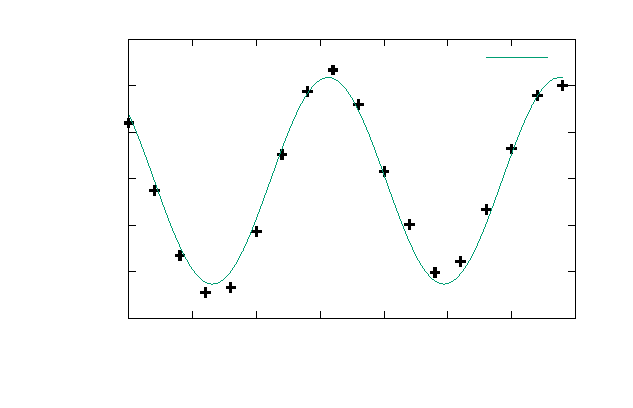
\includegraphics[width={288.00bp},height={180.00bp}]{malus_full}}%
    \gplfronttext
  \end{picture}%
\endgroup
 }
    \end{minipage} 
    \hfill
    \begin{minipage}[b]{.5\linewidth}
        \centering
        \captionsetup{labelformat=empty}
        \caption{b) pro $\lambda = 671$ nm}
        \resizebox{\textwidth}{!}{ % GNUPLOT: LaTeX picture with Postscript
\begingroup
  \makeatletter
  \providecommand\color[2][]{%
    \GenericError{(gnuplot) \space\space\space\@spaces}{%
      Package color not loaded in conjunction with
      terminal option `colourtext'%
    }{See the gnuplot documentation for explanation.%
    }{Either use 'blacktext' in gnuplot or load the package
      color.sty in LaTeX.}%
    \renewcommand\color[2][]{}%
  }%
  \providecommand\includegraphics[2][]{%
    \GenericError{(gnuplot) \space\space\space\@spaces}{%
      Package graphicx or graphics not loaded%
    }{See the gnuplot documentation for explanation.%
    }{The gnuplot epslatex terminal needs graphicx.sty or graphics.sty.}%
    \renewcommand\includegraphics[2][]{}%
  }%
  \providecommand\rotatebox[2]{#2}%
  \@ifundefined{ifGPcolor}{%
    \newif\ifGPcolor
    \GPcolorfalse
  }{}%
  \@ifundefined{ifGPblacktext}{%
    \newif\ifGPblacktext
    \GPblacktexttrue
  }{}%
  % define a \g@addto@macro without @ in the name:
  \let\gplgaddtomacro\g@addto@macro
  % define empty templates for all commands taking text:
  \gdef\gplbacktext{}%
  \gdef\gplfronttext{}%
  \makeatother
  \ifGPblacktext
    % no textcolor at all
    \def\colorrgb#1{}%
    \def\colorgray#1{}%
  \else
    % gray or color?
    \ifGPcolor
      \def\colorrgb#1{\color[rgb]{#1}}%
      \def\colorgray#1{\color[gray]{#1}}%
      \expandafter\def\csname LTw\endcsname{\color{white}}%
      \expandafter\def\csname LTb\endcsname{\color{black}}%
      \expandafter\def\csname LTa\endcsname{\color{black}}%
      \expandafter\def\csname LT0\endcsname{\color[rgb]{1,0,0}}%
      \expandafter\def\csname LT1\endcsname{\color[rgb]{0,1,0}}%
      \expandafter\def\csname LT2\endcsname{\color[rgb]{0,0,1}}%
      \expandafter\def\csname LT3\endcsname{\color[rgb]{1,0,1}}%
      \expandafter\def\csname LT4\endcsname{\color[rgb]{0,1,1}}%
      \expandafter\def\csname LT5\endcsname{\color[rgb]{1,1,0}}%
      \expandafter\def\csname LT6\endcsname{\color[rgb]{0,0,0}}%
      \expandafter\def\csname LT7\endcsname{\color[rgb]{1,0.3,0}}%
      \expandafter\def\csname LT8\endcsname{\color[rgb]{0.5,0.5,0.5}}%
    \else
      % gray
      \def\colorrgb#1{\color{black}}%
      \def\colorgray#1{\color[gray]{#1}}%
      \expandafter\def\csname LTw\endcsname{\color{white}}%
      \expandafter\def\csname LTb\endcsname{\color{black}}%
      \expandafter\def\csname LTa\endcsname{\color{black}}%
      \expandafter\def\csname LT0\endcsname{\color{black}}%
      \expandafter\def\csname LT1\endcsname{\color{black}}%
      \expandafter\def\csname LT2\endcsname{\color{black}}%
      \expandafter\def\csname LT3\endcsname{\color{black}}%
      \expandafter\def\csname LT4\endcsname{\color{black}}%
      \expandafter\def\csname LT5\endcsname{\color{black}}%
      \expandafter\def\csname LT6\endcsname{\color{black}}%
      \expandafter\def\csname LT7\endcsname{\color{black}}%
      \expandafter\def\csname LT8\endcsname{\color{black}}%
    \fi
  \fi
    \setlength{\unitlength}{0.0500bp}%
    \ifx\gptboxheight\undefined%
      \newlength{\gptboxheight}%
      \newlength{\gptboxwidth}%
      \newsavebox{\gptboxtext}%
    \fi%
    \setlength{\fboxrule}{0.5pt}%
    \setlength{\fboxsep}{1pt}%
    \definecolor{tbcol}{rgb}{1,1,1}%
\begin{picture}(5760.00,3600.00)%
    \gplgaddtomacro\gplbacktext{%
      \csname LTb\endcsname%%
      \put(814,704){\makebox(0,0)[r]{\strut{}$0.5$}}%
      \put(814,972){\makebox(0,0)[r]{\strut{}$1$}}%
      \put(814,1239){\makebox(0,0)[r]{\strut{}$1.5$}}%
      \put(814,1507){\makebox(0,0)[r]{\strut{}$2$}}%
      \put(814,1774){\makebox(0,0)[r]{\strut{}$2.5$}}%
      \put(814,2042){\makebox(0,0)[r]{\strut{}$3$}}%
      \put(814,2309){\makebox(0,0)[r]{\strut{}$3.5$}}%
      \put(814,2577){\makebox(0,0)[r]{\strut{}$4$}}%
      \put(814,2844){\makebox(0,0)[r]{\strut{}$4.5$}}%
      \put(814,3112){\makebox(0,0)[r]{\strut{}$5$}}%
      \put(814,3379){\makebox(0,0)[r]{\strut{}$5.5$}}%
      \put(946,484){\makebox(0,0){\strut{}$0$}}%
      \put(1577,484){\makebox(0,0){\strut{}$50$}}%
      \put(2208,484){\makebox(0,0){\strut{}$100$}}%
      \put(2839,484){\makebox(0,0){\strut{}$150$}}%
      \put(3470,484){\makebox(0,0){\strut{}$200$}}%
      \put(4101,484){\makebox(0,0){\strut{}$250$}}%
      \put(4732,484){\makebox(0,0){\strut{}$300$}}%
      \put(5363,484){\makebox(0,0){\strut{}$350$}}%
    }%
    \gplgaddtomacro\gplfronttext{%
      \csname LTb\endcsname%%
      \put(4376,3206){\makebox(0,0)[r]{\strut{}$I(\varphi)$}}%
      \csname LTb\endcsname%%
      \put(209,2041){\rotatebox{-270.00}{\makebox(0,0){\strut{}$\mu$A}}}%
      \put(3154,154){\makebox(0,0){\strut{}$\varphi$ $ (^{\circ})  $}}%
    }%
    \gplbacktext
    \put(0,0){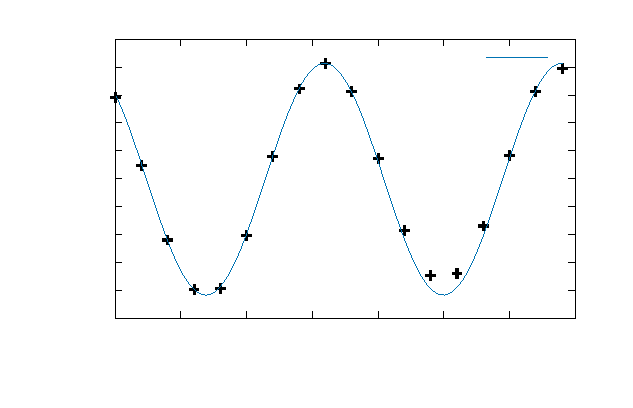
\includegraphics[width={288.00bp},height={180.00bp}]{malus_mono}}%
    \gplfronttext
  \end{picture}%
\endgroup
 }
    \end{minipage} 
    \captionsetup{type=graph}
    \caption{Závislost fotoproudu na úhlu natočení polarizátoru}
\end{table}

\section{Závěr}

Změřil jsem index lomu několika roztoků sacharózy a pomocí polarimetru zjistil jejich optickou stáčivost $ [\alpha] = 70.2 \pm 0.4 \ \ \frac{\text{cm}^{3}}{\text{g dm}} $. Tabulková hodnota je $ 66.53 $.

Podle Malusova zákona by intenzita světla po průchodu dvěma polarizátory natočenými o úhel $ \varphi $ měla sledovat vztah (3). Změřil jsem konstanty této závislosti $ I_{\text{max}} $ a $ I_{\text{min}} $ stejně jako samotnou intenzitu pro úhly v rozmezí $ [0^{\circ}, 360^{\circ}] $ a obě vynesl do grafu 1. Je vidět, že teoretická závislost opravdu sleduje tu změřenou, což ukazuje platnost tohoto zákona.

\begin{thebibliography}{0}
\bibitem{tabulky} Hustota pevných látek. Dostupné z~\url{http://www.converter.cz/tabulky/hustota-pevne.htmf}.   
\end{thebibliography}

\end{document}
